%%%%%%%%%%%%%%%%%%%%%%%%%%%%%%%%%%%%%%%%%%%%%%%%%%%%%%%%%%%%%%%%%%
\section{Wave-induced motion of a flexible vegetation stem}
\label{sec:flexveg}
%%%%%%%%%%%%%%%%%%%%%%%%%%%%%%%%%%%%%%%%%%%%%%%%%%%%%%%%%%%%%%%%%%

\noindent
The two preceding benchmarks verified the coupling against reference numerical solutions in single-phase channel flows. The final case applies it to a vegetation stem swaying under free-surface waves, which is the first validation against a physical experiment and the first use of the coupling in a two-phase setting, where the beam is driven by the orbital velocities of a propagating wave rather than by a unidirectional or uniformly oscillating channel flow. It is also the first case in which the structure barely confines the flow. The blade, $8~\mathrm{mm}$ wide in a flume $0.8~\mathrm{m}$ wide, blocks a small part of the flume cross-section, whereas the beam and the leaflet of the two channel benchmarks spanned $80\%$ of their simulated channel heights. Without that confinement the velocity approaching the stem stays close to the undisturbed wave kinematics, so the magnitude of the sampled velocity depends little on the sampling offset (Section~\ref{sec:flexveg_setup}). Flexible vegetation attenuates incident wave energy, modifies the mean flow and sediment transport within canopies, and is increasingly considered as a component of nature-based coastal defences, and predictive models for these processes rest on the ability to describe the motion of, and the force distribution along, an individual stem \citep{luhar_waveinduced_2016,jacobsen_waveinduced_2019}.

\noindent
The configuration reproduces the single-stem experiment of \citet{jacobsen_waveinduced_2019}, in which the motion of, and force on, individual plastic vegetation mimics under regular waves were measured in a laboratory wave flume. The data set suits the present purpose for three reasons. It provides the intra-wave kinematics along the entire stem rather than only at the tip, together with the base force and an estimate of the distributed loading, so the validation can interrogate the spatial structure of the coupled response. Its non-dimensional analysis classifies each test into quasi-static and dynamic response regimes, which allows the validation case to be chosen deliberately inside the range where the quasi-steady closure was shown to be accurate in Section~\ref{sec:leaflet_results}. And the authors derive measured drag coefficients from the experiment itself, so the coefficient required by the closure can be fixed a priori from published data. That transfer is possible only because of the weak confinement noted above, which is why the two channel benchmarks needed their own steady-CFD calibrations instead.

\subsection{Reference experiment and selection of the validation case}
\label{sec:flexveg_case_selection}
The experiment was performed in a wave flume at Delft University of Technology, $41.55~\mathrm{m}$ long, $0.8~\mathrm{m}$ wide and $0.9~\mathrm{m}$ deep, with a false bottom in the central test section accommodating a force transducer, so that the water depth was $0.65~\mathrm{m}$ at the wave paddle and $0.45~\mathrm{m}$ at the measuring location. A single stem was mounted on the transducer for each test, so the measurements characterise an isolated stem rather than a canopy. Surface elevation was recorded by seven wave gauges, the velocity with an electromagnetic flow meter traversed over the stem height, and the stem motion with a video camera at $25~\mathrm{Hz}$, giving the displacement along the stem at increments of $2.5~\mathrm{mm}$. Four plastic mimics were tested at two lengths under eight regular wave conditions, covering Cauchy numbers over five orders of magnitude.

\noindent
The present validation targets the blade labelled ``Mimic~3'' at the full length $l = 0.30~\mathrm{m}$, whose properties are listed in Table~\ref{tab:flexveg_properties}, under the wave condition designated H040T20. The choice is deliberate and follows directly from the modelling limitation quantified in the leaflet benchmark. \citet{jacobsen_waveinduced_2019} characterise the stem response by the Cauchy number, the Keulegan--Carpenter number and the relative stem length,
\begin{equation}
\label{eq:flexveg_nondim}
Ca = \frac{\rho\,\delta_y\,u_w^{2}\,l^{3}}{EI},
\qquad
KC = \frac{2\pi\,u_w}{\omega\,\delta_y},
\qquad
L = \frac{l\,\omega}{u_w},
\end{equation}
where $u_w$ is the characteristic depth-averaged root-mean-square orbital velocity and $\omega = 2\pi/T$ the cyclic wave frequency. The combination $CaL$ measures the ratio of hydrodynamic drag to elastic restoring stiffness, while $CaL/KC = (2/\pi^{2})(T_n\omega)^{2}$ controls whether the stem responds quasi-statically or dynamically. Following \citet{leclercq_reconfiguration_2018}, confirmed experimentally by \citet{jacobsen_waveinduced_2019}, the response is quasi-static, with the shape following the instantaneous force balance in a single spatial mode, for $CaL/KC < 0.20$, whereas larger values excite a dynamic response in which the added mass of the surrounding water amplifies the motion and introduces a second mode shape.

\noindent
This classification matches the range in which the present framework is accurate, since the closure of Eq.~\eqref{eq:almLineForce} carries no added-mass or history force and the leaflet benchmark showed that the framework under-predicts once fluid-inertia effects become dynamically significant. For Mimic~3 under H040T20 the measured characteristic velocity is $u_w = 7.7\times10^{-2}~\mathrm{m\,s^{-1}}$ and the orbital excursion is $a_w = u_w/\omega = 2.5\times10^{-2}~\mathrm{m}$, the natural length scale for the stem displacement throughout this section. These give $CaL/KC = 0.135$, inside the quasi-static regime, and the proper orthogonal decomposition reported in the reference confirms the placement, the motion being described entirely by the mean and a single mode. The inertia force reconstructed by the reference contributes less than $10\%$ of the maximum distributed force, so neglecting fluid inertia is justified a priori rather than assumed. By contrast the geometrically similar Mimic~2, a thinner blade of thickness $0.50~\mathrm{mm}$, gives $CaL/KC = 3.69$ under the same wave and would demand exactly the added-mass modelling that the present closure omits.

\noindent
One experimental artefact must be carried into the comparison. The reference reports a small negative mean deflection of this blade in stagnant water, attributed to anisotropic pre-tension introduced during manufacturing, which biases the mean position of the measured motion by about $-0.015\,l$ at the tip without affecting the oscillatory content. The comparison below therefore concentrates on the oscillation range and shape, and treats the mean offset as an acknowledged experimental bias.

\noindent
Three further wave conditions of the campaign are simulated with the same stem, summarised in Table~\ref{tab:flexveg_conditions}, chosen to span the widest range of forcing that remains defensible for the quasi-steady closure. H070T25 and H110T20 are quasi-static points at twice and three times the Keulegan--Carpenter number of the primary case, and H110T20 also drives the tip excursion to approximately one third of the stem length, which exercises the geometrically exact formulation at large deflection. H070T15 lies deliberately just \emph{beyond} the quasi-static limit at $CaL/KC = 0.241$ and probes where the drag-only closure stops being accurate. The two larger-amplitude conditions have Ursell numbers near $20$ and are generated with fifth-order Stokes kinematics \citep{fenton_fifth_1985}.

\begin{table}[!ht]
\centering
\small
\caption{The four simulated wave conditions (Mimic~3, $l = 0.30~\mathrm{m}$, $d = 0.45~\mathrm{m}$). Wave parameters and non-dimensional numbers follow Tables~1 and 3 of \citet{jacobsen_waveinduced_2019}, where $a_w$ and $u_w$ are the measured orbital excursion and characteristic velocity. $C_D$ is the drag-coefficient range fitted by the reference from the measured base force at each condition's $KC$, and $C_{dn}$ the value or values adopted for the actuator line.}
\label{tab:flexveg_conditions}
\footnotesize
\setlength{\tabcolsep}{3pt}
\renewcommand{\arraystretch}{1.15}
\begin{tabular}{l c c c c c c c c c c}
\toprule
Condition & $H$ (m) & $T$ (s) & Wave theory & $a_w$ (cm) & $u_w$ (cm/s) & $KC$ & $Ca$ & $CaL/KC$ & $C_D$ (meas.) & $C_{dn}$ \\
\midrule
H040T20 & $0.04$ & $2.0$ & Stokes II & $2.5$ & $7.7$  & $19.3$ & $0.21$ & $0.135$ & $3.5$--$4.0$ & $3.0$, $4.0$ \\
H070T15 & $0.07$ & $1.5$ & Stokes II & $2.7$ & $11.2$ & $20.9$ & $0.45$ & $0.241$ & $3.1$--$3.7$ & $4.0$ \\
H070T25 & $0.07$ & $2.5$ & Stokes V  & $5.0$ & $12.7$ & $39.7$ & $0.58$ & $0.088$ & $2.9$       & $3.0$ \\
H110T20 & $0.11$ & $2.0$ & Stokes V  & $7.0$ & $22.0$ & $55.1$ & $1.75$ & $0.137$ & $2.2$--$2.4$ & $2.4$ \\
\bottomrule
\end{tabular}
\end{table}

\subsection{Problem definition}
\label{sec:flexveg_geometry}
Figure~\ref{fig:flexVeg_schematic} presents the flume layout together with the computational domain. The bed is raised in the central test section by a $0.20~\mathrm{m}$ false bottom, flat at the paddle depth over the first $9.15~\mathrm{m}$, rising along a $2.20~\mathrm{m}$ ramp onto a $14.1~\mathrm{m}$ elevated plateau, and descending along a second ramp to a flat section, with a gently sloped porous absorber occupying the final $10.20~\mathrm{m}$. The computational domain reproduces the whole flume, spanning $41.55~\mathrm{m} \times 0.8~\mathrm{m} \times 1.1~\mathrm{m}$, with air above the still water level. The paddle section, both ramps, the plateau, and the absorber section are all meshed, so the wave shoals onto the plateau in the simulation as it does in the experiment, and the physical absorber is replaced by the numerical outlet absorption of Section~\ref{sec:theory_waves}. The simulation is three-dimensional throughout (Figure~\ref{fig:flexveg_domain}), and the schematic is drawn in side view because the motion is confined to the vertical plane of wave propagation. The stem is clamped at the mid-length of the plateau, $18.4~\mathrm{m}$ from the inlet and on the flume centreline, extending vertically to its free tip $0.15~\mathrm{m}$ below the still water level. The upstream fetch corresponds to approximately $4.7$ wavelengths of the target wave. The blade is represented by its centreline, with the rectangular cross-section entering through its area, second moment of area, and drag reference length as in the two preceding benchmarks, and the wide face normal to the wave direction, so the blade bends about its weak axis. The sensitivity of the coupled solution on this domain to the discretisation is examined in Appendix~\ref{app:flexveg_mesh}.

\begin{figure}[!htb]
\centering
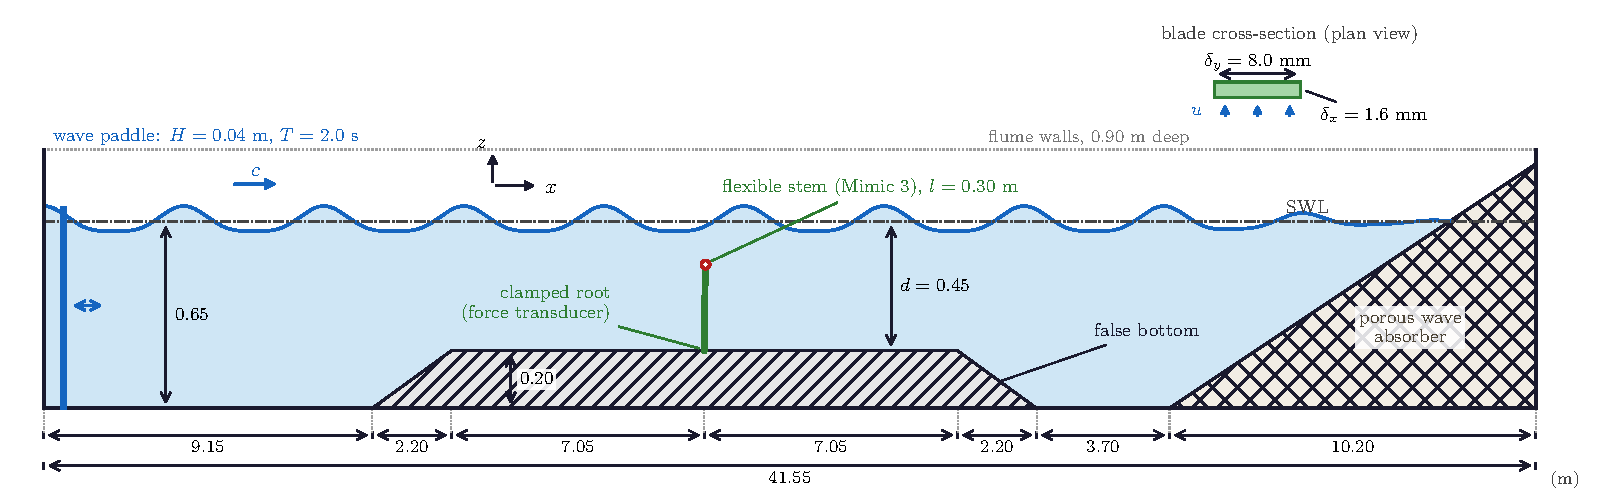
\includegraphics[width=0.95\textwidth]{flexVeg_schematic.pdf}
\caption{The flexible-vegetation validation problem in side view, with the vertical scale exaggerated and dimensions in metres, following Figure~1 of \citet{jacobsen_waveinduced_2019}. The $0.20~\mathrm{m}$ false bottom, accessed by $2.20~\mathrm{m}$ ramps, raises the bed in the central test section so that the still water depth is $0.65~\mathrm{m}$ at the paddle and $d = 0.45~\mathrm{m}$ over the $14.1~\mathrm{m}$ plateau. The Mimic~3 blade is clamped at the plateau centre. The computational domain reproduces the whole flume and is three-dimensional. The inset shows the blade cross-section in plan view, with the wide face $\delta_y$ normal to the wave direction.}
\label{fig:flexVeg_schematic}
\end{figure}

\noindent
The case is solved with the two-phase formulation of Section~\ref{sec:fluidSubsystem}, using the volume-of-fluid phase fraction to capture the free surface and the modified pressure $p_{\mathrm{rgh}}$ as the pressure variable, as implemented in the \texttt{interFoam} solver of OpenFOAM. At the inlet, a regular wave of the appropriate order is imposed through the boundary conditions of Section~\ref{sec:theory_waves}, with active absorption so that reflected waves are not re-injected \citep{higuera_realistic_2013} and the amplitude ramped up smoothly over the first two wave periods, and at the outlet a shallow-water absorption condition dissipates the outgoing wave. The bed is a stationary no-slip wall on which the stem root is clamped, the top boundary is open to the atmosphere at fixed total pressure, and the two lateral boundaries represent the flume side walls. The fluid is initialised at rest with a hydrostatic pressure distribution and a flat interface at the still water level, and the stem starts undeformed, so the flow at the stem is not yet periodic when the run begins and all quantitative comparisons are taken from the end of the run. The blade is close to neutrally buoyant, so gravity and buoyancy nearly cancel along the stem and the response is dominated by the balance between hydrodynamic drag and elastic restoring moment.

\begin{table}[!ht]
\centering
\small
\caption{Physical parameters of the flexible-vegetation validation case, following \citet{jacobsen_waveinduced_2019} (Mimic~3, $l = 0.30~\mathrm{m}$, wave condition H040T20).}
\label{tab:flexveg_properties}
\setlength{\tabcolsep}{6pt}
\renewcommand{\arraystretch}{1.15}
\begin{tabular}{l c l}
\toprule
Quantity & Symbol & Value \\
\midrule
\multicolumn{3}{l}{\textbf{Wave and flume}} \\
\cmidrule(lr){1-3}
Wave height (target)             & $H$    & $0.04~\mathrm{m}$ \\
Wave period                      & $T$    & $2.0~\mathrm{s}$ \\
Still water depth (test section) & $d$    & $0.45~\mathrm{m}$ \\
Water density                    & $\rho$ & $1.0\times10^{3}~\mathrm{kg\,m^{-3}}$ \\
Kinematic viscosity              & $\nu$  & $1.0\times10^{-6}~\mathrm{m^{2}\,s^{-1}}$ \\
Characteristic orbital velocity  & $u_w$  & $7.7\times10^{-2}~\mathrm{m\,s^{-1}}$ \\
Orbital excursion                & $a_w$  & $2.5\times10^{-2}~\mathrm{m}$ \\
\midrule
\multicolumn{3}{l}{\textbf{Stem (Mimic~3)}} \\
\cmidrule(lr){1-3}
Length                           & $l$        & $0.30~\mathrm{m}$ \\
Blade width (facing the wave)    & $\delta_y$ & $8.0\times10^{-3}~\mathrm{m}$ \\
Blade thickness                  & $\delta_x$ & $1.6\times10^{-3}~\mathrm{m}$ \\
Young's modulus                  & $E$        & $2.2\times10^{9}~\mathrm{Pa}$ \\
Solid density                    & $\rho_s$   & $1.09\times10^{3}~\mathrm{kg\,m^{-3}}$ \\
Bending stiffness                & $EI$       & $6.0\times10^{-3}~\mathrm{N\,m^{2}}$ \\
Natural period (submerged)       & $T_n$      & $0.26~\mathrm{s}$ \\
\bottomrule
\end{tabular}
\end{table}

\subsection{Choice of the drag coefficient}
\label{sec:flexveg_cd}
The steady-CFD calibration used in the two channel benchmarks is not transferable here, because the flow past the blade is oscillatory and depth-varying and a steady rigid-plate simulation in a wave flume has no meaningful steady state. The reference experiment supplies the coefficient instead. \citet{jacobsen_waveinduced_2019} derive the average drag coefficient for each mimic by least-squares fitting of the measured base force to the relative-velocity Morison formulation integrated over the instantaneous stem shape, and report it against the Keulegan--Carpenter number, the fitted forces reproducing the measured forces generally within $10$ to $20\%$. At $KC = 19.3$, the two repeat tests of the present blade yield $C_D = 3.5$ and $4.0$, with the neighbouring cluster for the shorter $l = 0.15~\mathrm{m}$ specimen lying slightly lower at $3.2$ to $3.3$.

\noindent
Rather than committing to a single reading, the primary case is simulated twice, at $C_{dn} = 3.0$ and $4.0$. The upper value is the upper repeat fit of the present blade, whereas $3.0$ sits slightly \emph{below} the blade's own fitted cluster and is retained as a deliberately conservative lower bracket, so the pair brackets the family of published fitted values and this propagated range appears explicitly in every comparison that follows. The drag reference length is the blade width. For the three additional conditions the coefficient is read from the same figure at each condition's $KC$ (Table~\ref{tab:flexveg_conditions}). For H070T25 and H110T20 the adopted values match the fitted clusters, at $3.0$ against $2.85$ to $2.94$, marginally above within reading accuracy, and $2.4$ inside $2.2$ to $2.4$. For the boundary probe H070T15 the upper reading of the primary case is retained even though it lies marginally above that condition's own cluster of $3.1$ to $3.7$, a deliberately generous choice made so that any shortfall observed at the boundary of the quasi-static regime cannot be attributed to a conservative drag input.

\noindent
The tangential coefficient is fixed at $C_{dt} = 0.01$ as before, which matters little because the stem stays close to vertical while the wave-induced velocity is predominantly horizontal, so the relative velocity is nearly normal to the blade axis throughout the cycle. No recalibration of either coefficient against the measured stem motion is performed. The drag coefficients are fixed from the published fits and the coupling-operator settings are carried over from the channel benchmarks, so the comparison is blind with respect to the validation data, with the operator settings inherited rather than independently derived. One additional simulation at $C_{dn} = 5.0$, deliberately \emph{outside} the measured band, is reported below purely as a sensitivity diagnostic, to test whether a coefficient above the measured band could make up a shortfall in the response amplitude, and it is never used as a calibration.

\subsection{Numerical set-up}
\label{sec:flexveg_setup}

\noindent
The fluid domain is discretised with a structured hexahedral mesh of approximately $1.35\times10^{7}$ cells, built in six blocks spanning the whole flume with the \texttt{blockMesh} utility of OpenFOAM, with $20$ cells across the width and $220$ in the vertical. Over the plateau the streamwise spacing is uniform at $\Delta x = 6~\mathrm{mm}$, with $\Delta y = 40~\mathrm{mm}$ across the flume and $\Delta z = 4.1~\mathrm{mm}$ in the vertical. Away from the plateau the streamwise spacing is graded from $6~\mathrm{mm}$ at the plateau edges to $32~\mathrm{mm}$ over the paddle section and about $200~\mathrm{mm}$ at the outlet, so the wave is resolved finely where it is measured and the mesh coarsens where it is not. Figure~\ref{fig:flexveg_domain} shows the three-dimensional domain together with a close-up of the mesh near the stem. The vertical resolution corresponds to about $10$ cells per wave height for the primary condition, rising to $27$ for the largest wave, and the streamwise spacing over the plateau to about $650$ cells per wavelength. \citet{larsen_performance_2019} propagated a nonlinear regular wave with the same solver family and found that $12.5$ cells per wave height carried it over about five wavelengths without appreciable decay provided the Courant number was kept near $0.05$, whereas $6.25$ cells per wave height smeared the interface. The primary condition lies between these values, the larger waves are resolved more finely than either, the celerity-based Courant number here is about $0.016$, and the upstream fetch is close to the propagation distance over which that assessment was made. The adequacy of the resolution is shown directly in Section~\ref{sec:flexveg_results_wave} by comparing the achieved elevation and orbital velocities at the stem against the measured values, which is the sharper test because it checks the quantity that actually drives the stem, and Appendix~\ref{app:flexveg_mesh} repeats the largest-deflection condition on meshes a factor of $\sqrt{2}$ coarser and finer in every direction, where the load and the response move by about $2\%$.

\begin{figure}[!htb]
\centering
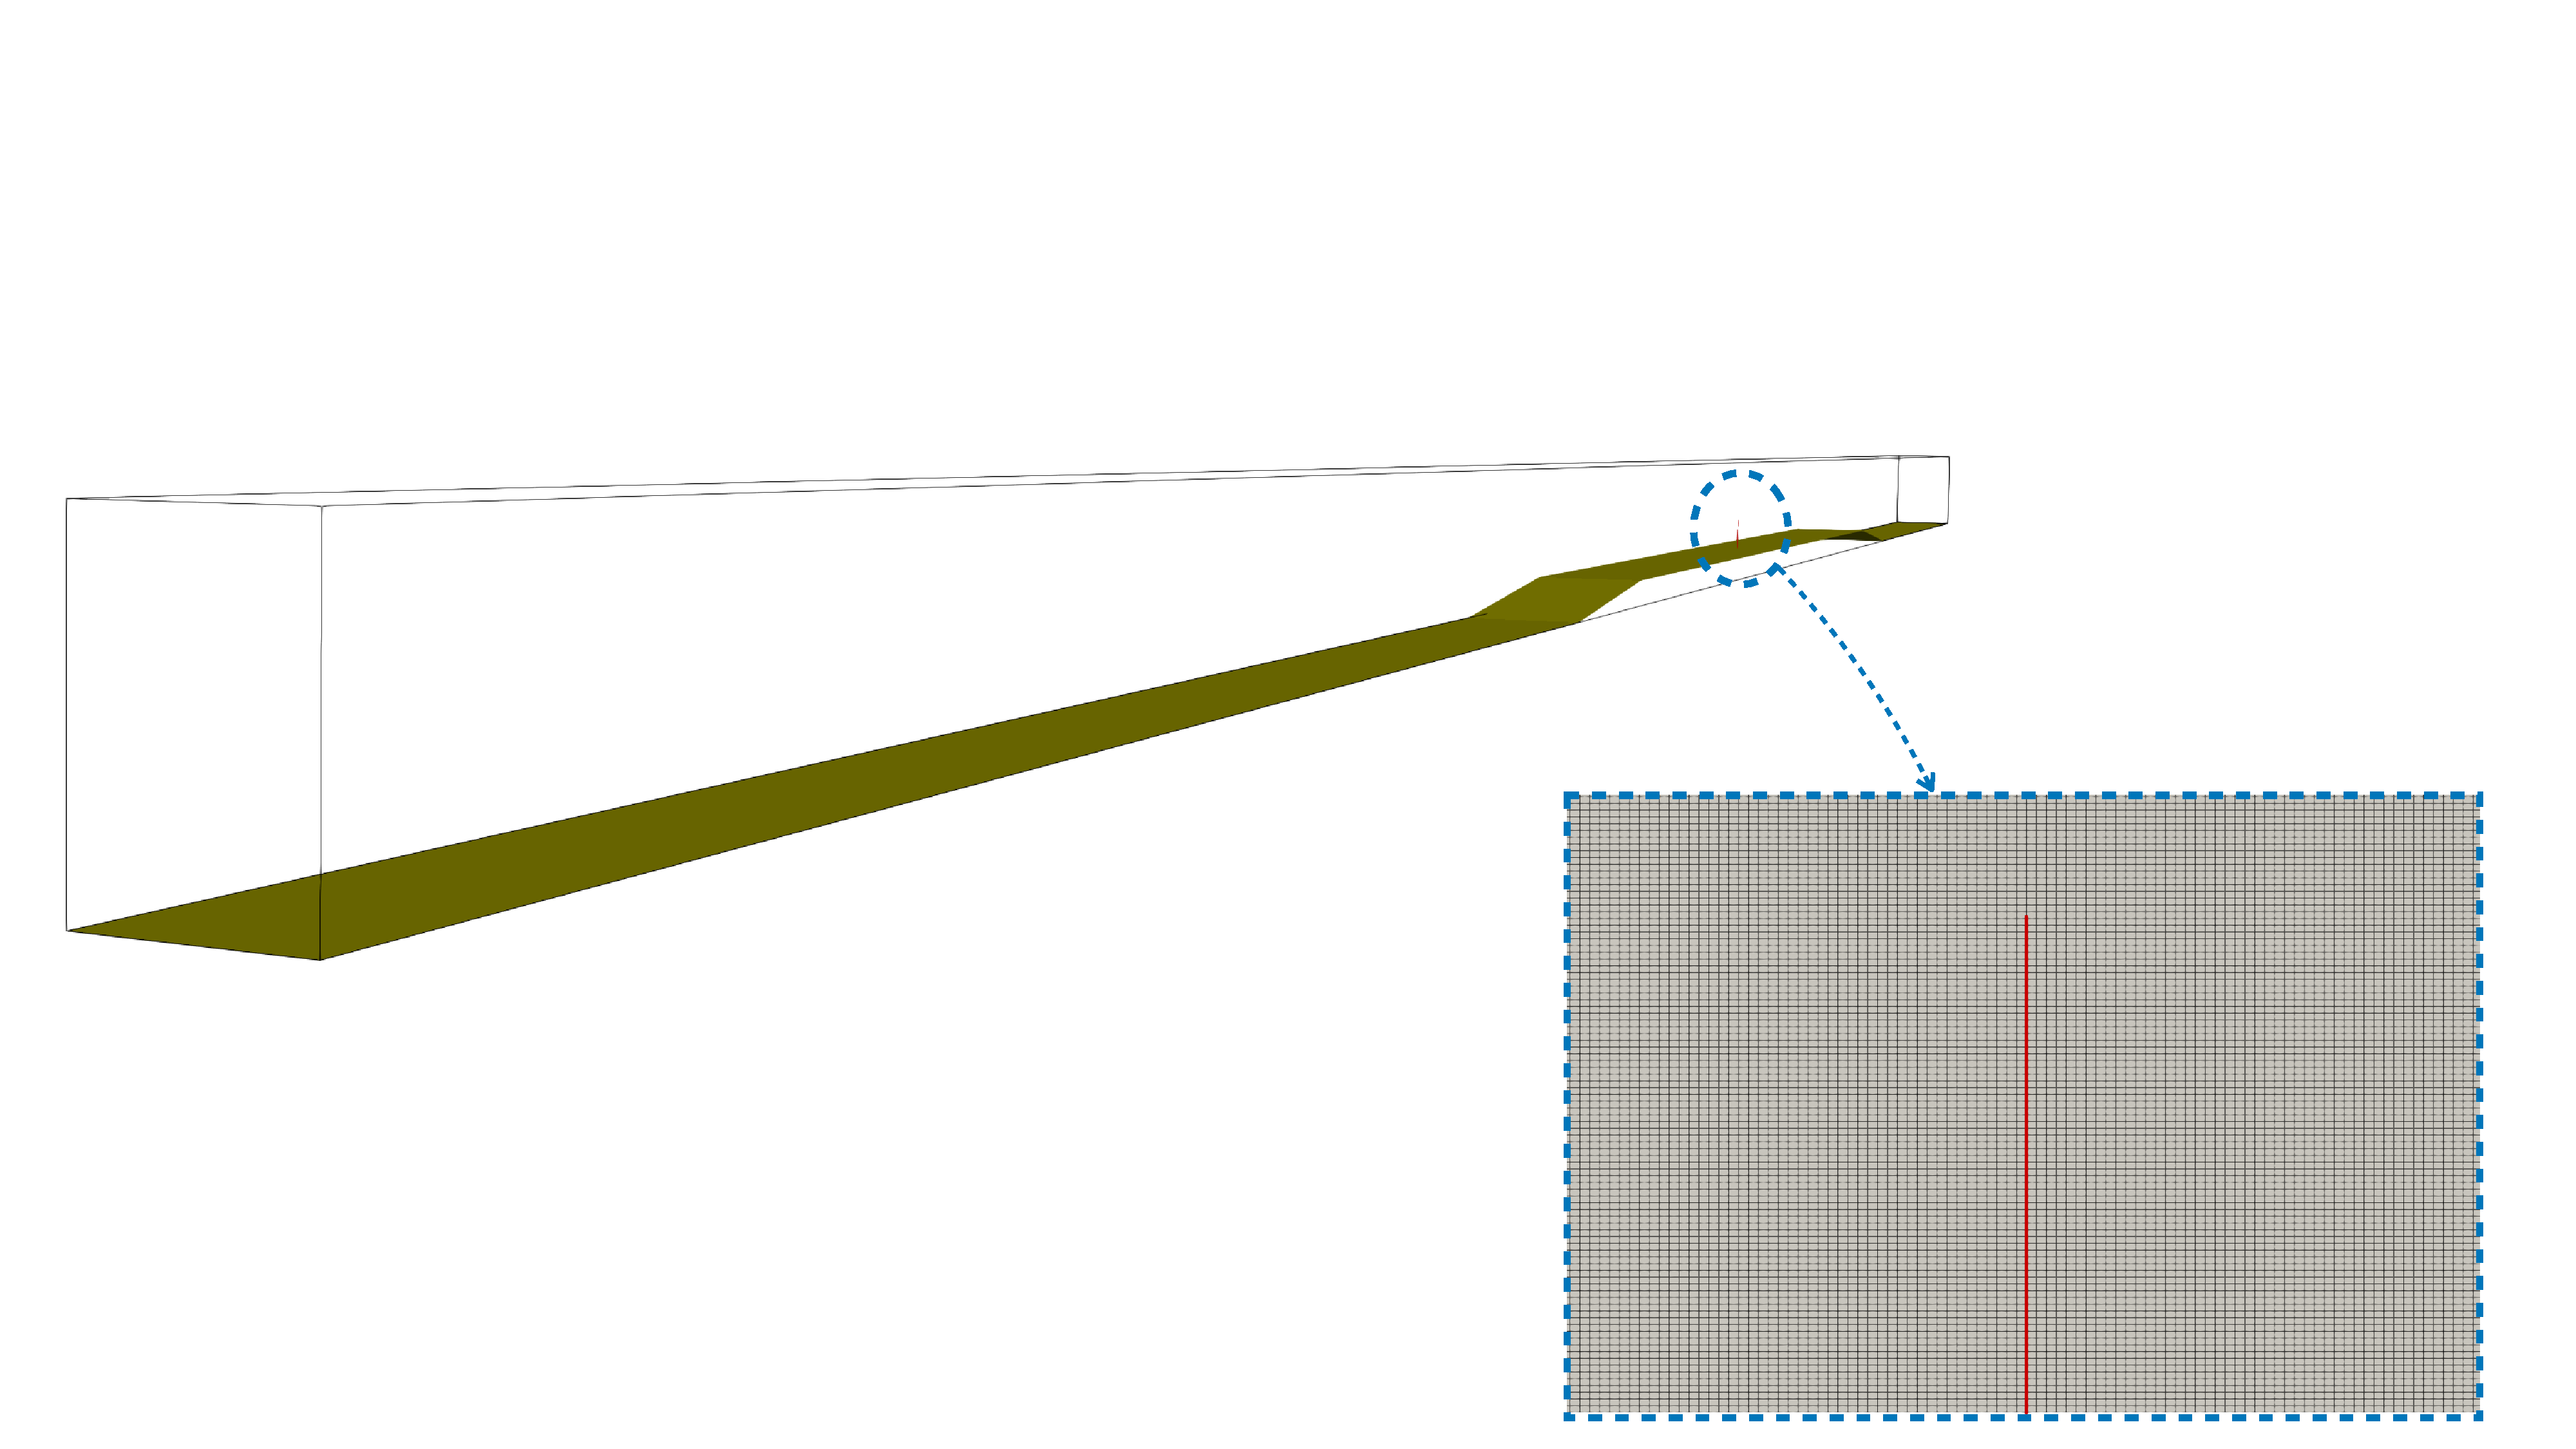
\includegraphics[width=0.95\textwidth,trim={20 5 40 310},clip]{flexVeg_3dDomain.pdf}
\caption{Snapshot of the three-dimensional computational domain of the wave flume, with the bed and the false bottom shaded and the stem shown in red. The dashed circle marks the stem region, and the inset is a close-up of the mesh near the stem in a vertical plane through the stem.}
\label{fig:flexveg_domain}
\end{figure}

\noindent
The beam is discretised into $60$ finite volume segments, consistent with the beam-mesh study of Section~\ref{sec:beamtunnel_sensitivity}, and the adequacy of that resolution for the present load distribution is confirmed independently by the quasi-static test of Section~\ref{sec:flexveg_conditions}. The kernel width is $\varepsilon = 2.5\,\Delta x = 0.015~\mathrm{m}$, sized by the same rule adopted in the channel benchmarks, and the upstream sampling is performed $0.375~\mathrm{m}$ upstream of each beam segment in the wave propagation direction, projected onto the vertical plane through the stem. That offset places the sampled velocity outside the momentum-sink region, but it is a nonlocal input in a propagating wave, corresponding to about a tenth of the local wavelength, so the sampled kinematics lead the at-stem wave by a known phase $k \times 0.375~\mathrm{m}$, approximately $35^{\circ}$ for the primary condition and evaluated per condition. Two properties keep this admissible. The offset affects phase but not magnitude, since the wave propagates over a flat plateau without decay and the sampled orbital-velocity amplitude was verified to match the at-stem amplitude to within a few percent. The phase lead is also deterministic and is corrected for wherever phase enters a comparison. The absolute phase of the response relative to the local wave is therefore not claimed as an independently validated quantity, and the internal phase consistency of the coupled solution is certified instead by the in-phase quasi-static reconstruction of Section~\ref{sec:flexveg_conditions}. A dedicated sampling-distance sweep was not repeated in the wave flume, the sensitivity to that distance having been quantified in Section~\ref{sec:beamtunnel_sensitivity}, and this transfer is acknowledged as a limitation.

\noindent
The simulation is advanced with a fixed time step of $\Delta t = 5\times10^{-5}~\mathrm{s}$, which is $4\times10^{4}$ steps per wave period and well below the interface-Courant limit. The small step is dictated by the robustness of the beam Newton solve within the partitioned coupling rather than by the fluid, for the reason given in Section~\ref{sec:almParallelSearch}, so the run time is set by the structural solve. Each case simulates $32~\mathrm{s}$ of physical time, sixteen wave periods at the primary condition, and all results below are extracted from the final three periods, over which the per-period tip-displacement extrema vary by less than $1\%$ in every run. That repeatability is what establishes that the start-up is over.

\subsection{Wave-field verification at the stem}
\label{sec:flexveg_results_wave}
Any error in the local wave kinematics propagates quadratically into the drag force, so the generated wave is verified at the stem location first. Figure~\ref{fig:flexveg_wave} shows the simulated surface elevation over two developed wave periods for all four conditions, against the crest and trough elevations measured at the same location, and Table~\ref{tab:flexveg_wave_check} complements it with the vertical-profile quantities that drive the stem, namely the crest and trough horizontal orbital velocities averaged over the stem height and the characteristic velocity $u_w$.

\begin{figure}[!htb]
\centering
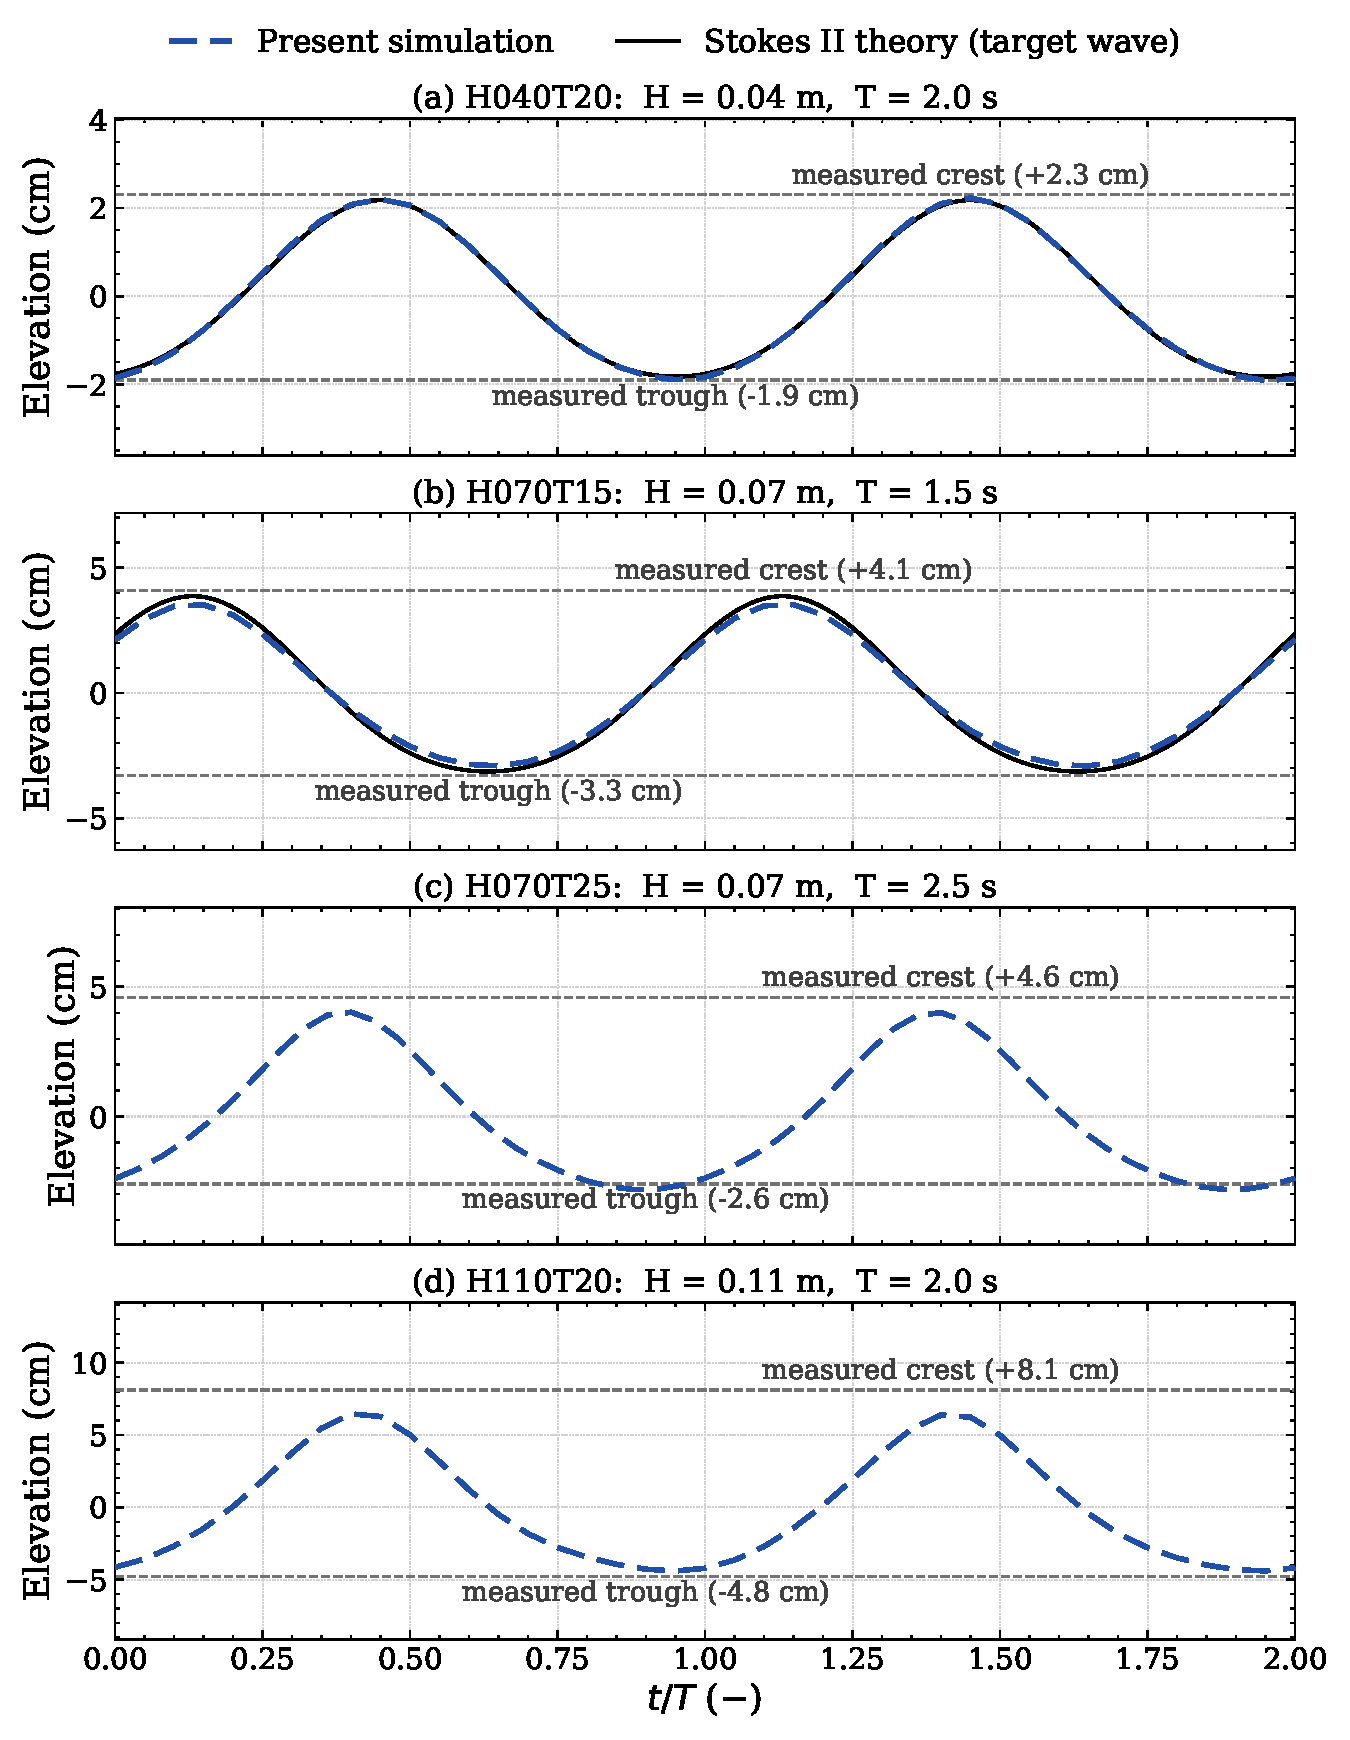
\includegraphics[width=0.78\textwidth]{mimic3_wave_elevation.pdf}
\caption{Verification of the wave field at the stem location for the four simulated conditions. Surface elevation over two developed wave periods, about the local mean water level, against the crest and trough elevations measured at the same location \citep[Table~1]{jacobsen_waveinduced_2019}, and, for the Stokes~II cases (a, b), against second-order theory at the target wave height. The measured values describe the \emph{achieved} experimental wave while the simulation generates the target wave, and both heights are listed in Table~\ref{tab:flexveg_wave_check}.}
\label{fig:flexveg_wave}
\end{figure}

\begin{table}[!ht]
\centering
\small
\caption{Wave kinematics at the stem location, simulation against the measurements reported in Tables~1 and 3 of \citet{jacobsen_waveinduced_2019}. The first pair of columns gives the wave height each simulation was driven at and the height the flume achieved, because the two differ and the remaining columns therefore describe slightly different waves. $\eta_c$ and $\eta_t$ are the crest and trough elevations, $\langle \tilde{u}_c \rangle_z$ and $\langle \tilde{u}_t \rangle_z$ the crest and trough horizontal orbital velocities averaged over the stem height, and $u_w$ the characteristic orbital velocity.}
\label{tab:flexveg_wave_check}
\footnotesize
\setlength{\tabcolsep}{3.5pt}
\renewcommand{\arraystretch}{1.15}
\begin{tabular}{l cc cc cc cc cc cc}
\toprule
 & \multicolumn{2}{c}{$H$ (cm)} & \multicolumn{2}{c}{$\eta_c$ (cm)} & \multicolumn{2}{c}{$\eta_t$ (cm)} & \multicolumn{2}{c}{$\langle \tilde{u}_c \rangle_z$ (cm/s)} & \multicolumn{2}{c}{$\langle \tilde{u}_t \rangle_z$ (cm/s)} & \multicolumn{2}{c}{$u_w$ (cm/s)} \\
\cmidrule(lr){2-3}\cmidrule(lr){4-5}\cmidrule(lr){6-7}\cmidrule(lr){8-9}\cmidrule(lr){10-11}\cmidrule(lr){12-13}
Condition & target & achieved & sim & meas & sim & meas & sim & meas & sim & meas & sim & meas \\
\midrule
H040T20 & $4.0$  & $4.1$  & $+2.3$ & $+2.3$ & $-1.9$ & $-1.9$ & $+8.0$  & $+8.0$  & $-7.3$  & $-7.3$  & $7.7$  & $7.7$ \\
H070T15 & $7.0$  & $7.4$  & $+3.5$ & $+4.1$ & $-2.9$ & $-3.3$ & $+13.4$ & $+11.5$ & $-12.8$ & $-10.8$ & $13.1$ & $11.2$ \\
H070T25 & $7.0$  & $7.2$  & $+4.0$ & $+4.6$ & $-2.8$ & $-2.6$ & $+15.7$ & $+15.6$ & $-12.1$ & $-9.9$  & $14.0$ & $12.7$ \\
H110T20 & $11.0$ & $12.9$ & $+6.5$ & $+8.1$ & $-4.4$ & $-4.8$ & $+21.4$ & $+25.4$ & $-16.9$ & $-19.1$ & $19.3$ & $22.0$ \\
\bottomrule
\end{tabular}
\end{table}

\noindent
For the primary condition the agreement is essentially exact. The simulated elevation follows the second-order theory curve, the crest and trough match the measured values to within $0.05~\mathrm{cm}$, and every velocity measure agrees to within $1\%$, including the Stokes-II asymmetry between the stronger, shorter crest phase and the weaker, longer trough phase and the small negative Eulerian mean at the stem. The wave that drives the primary validation is therefore the experimental wave, and any discrepancy in the stem response cannot be attributed to the wave field. The tabulated values are those of the $C_{dn} = 3.0$ run; in the $C_{dn} = 4.0$ run the crest velocity at the stem is $7.68$ instead of $8.0~\mathrm{cm\,s^{-1}}$, about $4\%$ lower, because the stronger momentum sink slows the flow locally. That difference is the two-way coupling acting on the wave it sees, not a defect in the wave generation. The simulated mean water level sits $0.7$ to $0.9~\mathrm{cm}$ above the still water level in all runs, a constant set-up associated with the mass injected during the inlet ramp that the outlet absorption maintains but does not drain. It is steady over the entire analysis window and elevations are reported about the local mean, exactly as a wave gauge reports them, and a depth increase of $0.8~\mathrm{cm}$ on $0.45~\mathrm{m}$ shifts the wavenumber and the orbital-velocity amplitude by of the order of $1\%$, an order of magnitude below the response deficits under discussion.

\noindent
For the three additional conditions the comparison must separate model error from a mismatch of inputs, because the simulation generates the \emph{target} wave of each condition whereas the published kinematics describe the \emph{achieved} flume wave. For H110T20 the flume overshot its target substantially, at $12.9~\mathrm{cm}$ against $11~\mathrm{cm}$, so the simulated crest and orbital velocities sit systematically below the measured ones by essentially that margin, the velocity ratio matching the height ratio almost exactly. The opposite arises for H070T15, where the simulated velocities \emph{exceed} the measurement by about $17\%$ even though the simulated crest is low. At this condition the relative depth is $kd \approx 1.04$, at the edge of validity of the shallow-water outlet absorption, and the partial reflection creates a weak standing-wave pattern that raises the velocity locally at the stem while lowering the elevation. The contamination can be estimated from its own signature, the crest sitting about $14\%$ below the measured value while the velocity sits about $17\%$ above it. That is the pattern of a partial standing wave sampled near an elevation node and velocity antinode, and it implies an amplitude reflection coefficient of the order of $0.15$, an order of magnitude larger than the few-percent pattern detectable at the other conditions. This contaminates the local wave rather than the wave generation, and it is the second of two grounds on which this condition is excluded from the quantitative closure-accuracy claim below. H070T25 sits in between, with crest velocity matching the measurement and a trough somewhat too strong.

\subsection{Stem motion along the blade}
\label{sec:flexveg_results_motion}
Figure~\ref{fig:flexveg_alongblade} compares the simulated stem motion over one wave period against the video-tracked displacement of the experiment, for both ends of the propagated coefficient range and for the out-of-band sensitivity value $C_{dn} = 5.0$. The compared quantity is the horizontal displacement $x_s$ of the centreline, normalised by the stem length, at the four stations $s/l = 0.25$, $0.50$, $0.75$ and $1.00$ tracked in the experiment, where $s$ is the arc-length from the clamped root. Because the upstream sampling shifts the phase of the whole response relative to the local wave, each run is aligned in time by its tip peak, with one shift per run applied at all four stations, so the relative phasing along the blade is preserved and remains a genuine prediction.

\begin{figure}[!htb]
\centering
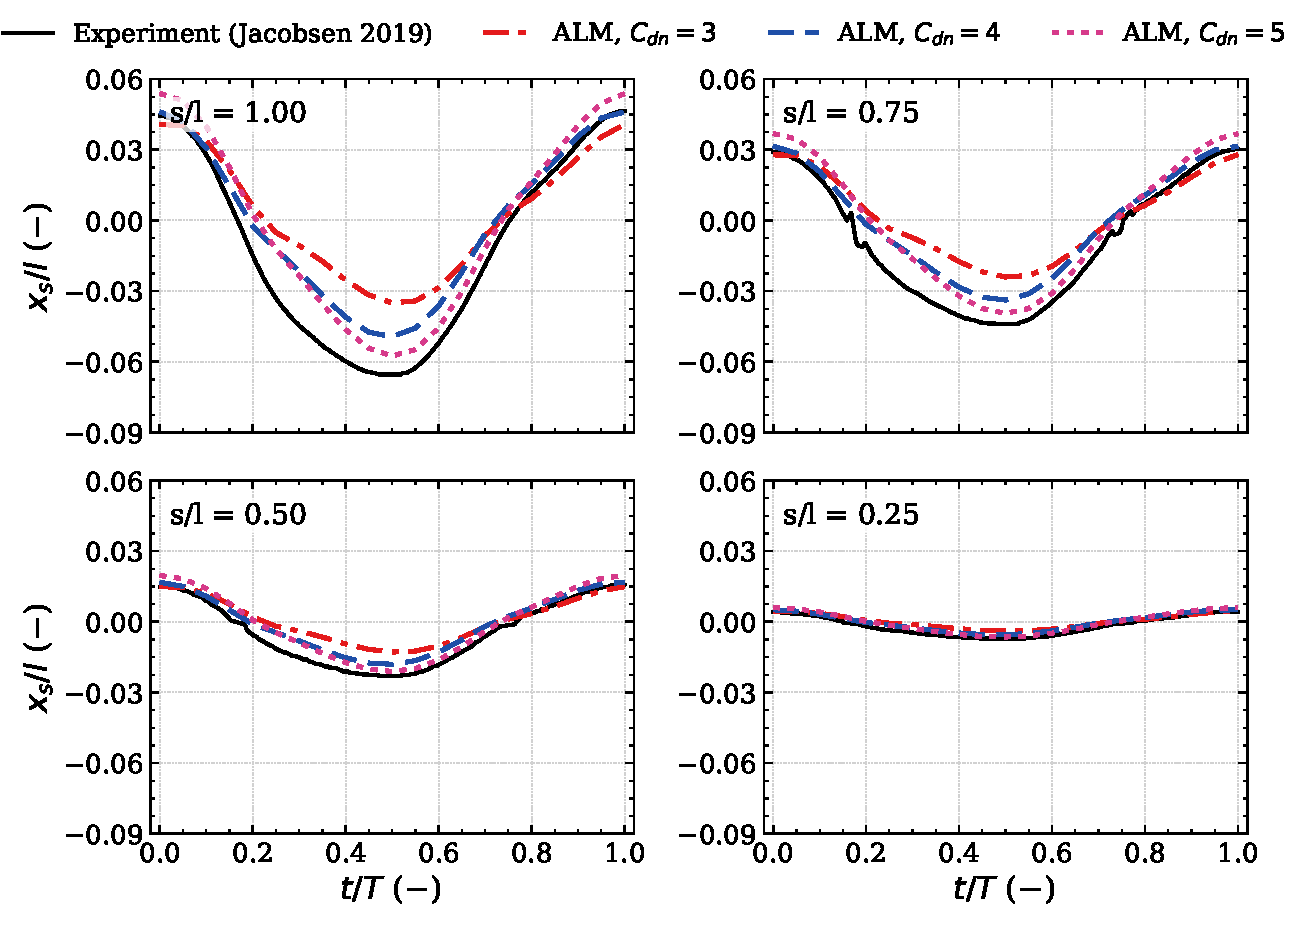
\includegraphics[width=0.95\textwidth]{mimic3_alongblade_timeseries.pdf}
\caption{Horizontal stem displacement over one wave period at four stations along the blade. Present two-way simulations at $C_{dn} = 3.0$ and $4.0$, the propagated coefficient range bracketing the published fitted values, and at the out-of-band sensitivity value $C_{dn} = 5.0$, against the video-tracked measurement of \citet[Figure~14d]{jacobsen_waveinduced_2019}. Each run is aligned in time by its tip peak, with one shift per run applied at all stations. The experimental curves carry the $-0.015\,l$ pre-tension mean offset, which deepens their troughs.}
\label{fig:flexveg_alongblade}
\end{figure}

\noindent
At every station the simulated motion reproduces the shape of the measured signal, including the sawtooth asymmetry between the fast forward sweep under the crest and the slower backward relaxation under the trough, the simultaneous motion of all four stations that characterises the single-mode quasi-static response, and the monotonic growth of amplitude from root to tip. A proper orthogonal decomposition of the simulated motion attributes $100.0\%$ of the fluctuation energy to a single spatial mode, exactly as the reference reports for the measurement. At $C_{dn} = 4.0$ the positive tip peak matches the measurement to within $1\%$, at $+13.9~\mathrm{mm}$ against $+14.0~\mathrm{mm}$. The measured troughs are deeper than the simulated ones at all stations, most of that difference being the documented pre-tension offset, which shifts the whole measured signal by about $-4.5~\mathrm{mm}$, and the remainder the amplitude shortfall quantified next.

\noindent
The peak-to-trough oscillation range, which is unaffected by the mean offset and is therefore the cleanest scalar measure, is shown in Figure~\ref{fig:flexveg_range_envelope}(a) as a profile along the blade normalised by $a_w$. The two runs of the propagated range bracket the response, capturing $68$ to $72\%$ of the measured range at $C_{dn} = 3.0$ and $85$ to $89\%$ at $4.0$, depending on station. These station-level fractions are referenced to the time-resolved series of Figure~14d of the reference, whose tip range of $1.34\,a_w$ is slightly smaller than the $1.41\,a_w$ of the compilation across conditions in their Figure~5, which gives tip fractions of $65\%$ and $81\%$ instead. Both normalisations appear in this section and are always identified, and the summary statement of $65$ to $89\%$ used elsewhere spans the two coefficients, the four stations, and the two experimental references. Two features of the profile carry more information than the percentages. The captured fraction is nearly constant along the blade, so the simulated \emph{mode shape} is correct at both coefficients and the entire deficit is a single amplitude factor. The response also grows visibly slower than linearly with the coefficient, a $33\%$ increase of $C_{dn}$ yielding a $26\%$ increase of range, because the stem follows the water more closely as the drag grows and the stronger momentum sink weakens the local flow, so no coefficient inside the measured band can close the residual gap.

\begin{figure}[!htb]
\centering
\begin{subfigure}[b]{0.53\textwidth}
  \centering
  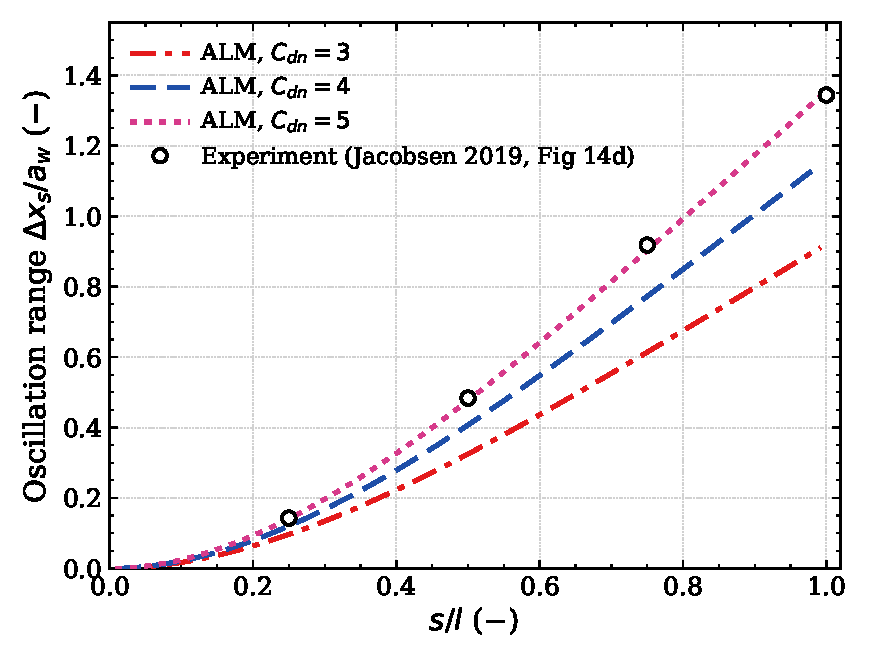
\includegraphics[width=\linewidth]{mimic3_range_profile.pdf}
  \caption{}
\end{subfigure}\hfill
\begin{subfigure}[b]{0.45\textwidth}
  \centering
  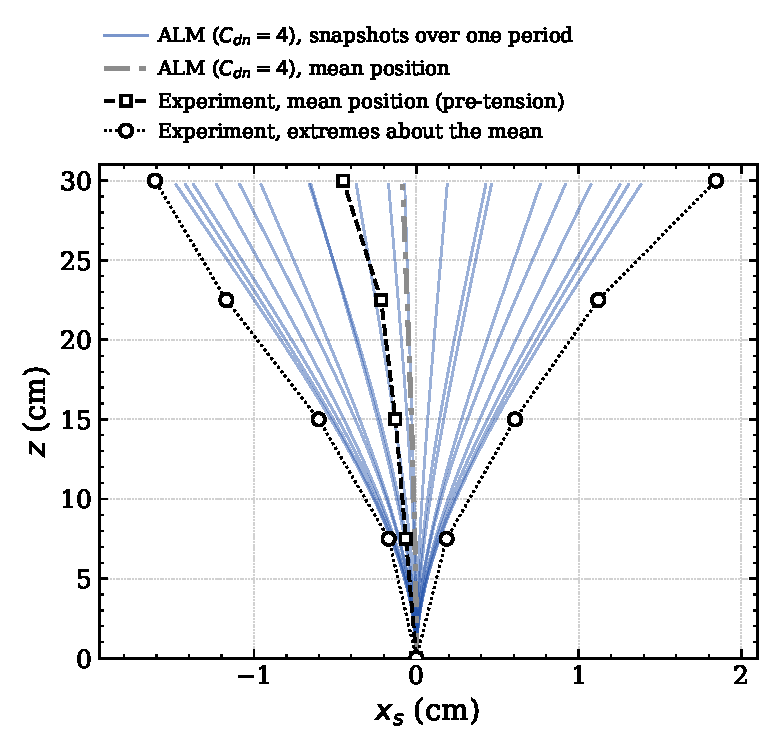
\includegraphics[width=\linewidth]{mimic3_envelope.pdf}
  \caption{}
\end{subfigure}
\caption{(a) Peak-to-trough oscillation range of the horizontal displacement along the blade, normalised by the wave excursion $a_w$, for the three simulations against the four digitised experimental stations. The captured fraction is nearly uniform along the blade, so the simulated mode shape is exact and the residual deficit is a single amplitude factor. (b) Swaying envelope at $C_{dn} = 4.0$, showing stem centrelines at twenty equispaced instants of one wave period and the time-mean position, compared with the experiment reconstructed from the four digitised stations of \citet[Figure~14d]{jacobsen_waveinduced_2019}: the measured mean position (squares), which carries the $-0.015\,l$ static pre-tension offset of the physical blade, and the measured extreme-phase positions referenced about that mean (circles), which is the like-for-like comparison with an unbiased model.}
\label{fig:flexveg_range_envelope}
\end{figure}

\noindent
The envelope of Figure~\ref{fig:flexveg_range_envelope}(b) completes the kinematic comparison, with the experiment reconstructed in two separate parts. The first is the experimental \emph{mean} position, which leans backward with a tip offset of $-4.5~\mathrm{mm}$, the static pre-tension of the physical blade that no unbiased model reproduces. The simulated mean position is essentially vertical, which is the expected quasi-static result, since a symmetric oscillatory drag produces no rectified mean deflection at this order. The second part is the experimental extreme-phase configurations referenced \emph{about that mean}, with no measured value altered, and on this basis the envelopes agree closely. The simulated fan is forward-backward asymmetric in the same sense as the experiment, because the longer trough phase of the second-order wave acts on the stem for a larger fraction of the period, its extremes track the mean-referenced experimental extremes along the entire blade, and the residual difference is the $85$ to $89\%$ oscillatory amplitude fraction already quantified.

\subsection{Distributed hydrodynamic force}
\label{sec:flexveg_force}
The experiment makes the force distribution accessible in two forms, namely a distributed total force along the stem reconstructed from the tracked motion and the calibrated structural model, and the internal shear derived from it, whose value at the root is anchored by the transducer measurement. Figure~\ref{fig:flexveg_heatmaps} shows the corresponding quantities of the $C_{dn} = 4.0$ simulation as space--time maps over four wave periods, drawn with the colour scales of the reference figures, which are reproduced alongside for direct comparison.

\noindent
\hl{FIGURE REUSE PERMIT}

\begin{figure}[!htb]
\centering
\begin{subfigure}[b]{0.49\textwidth}
  \centering
  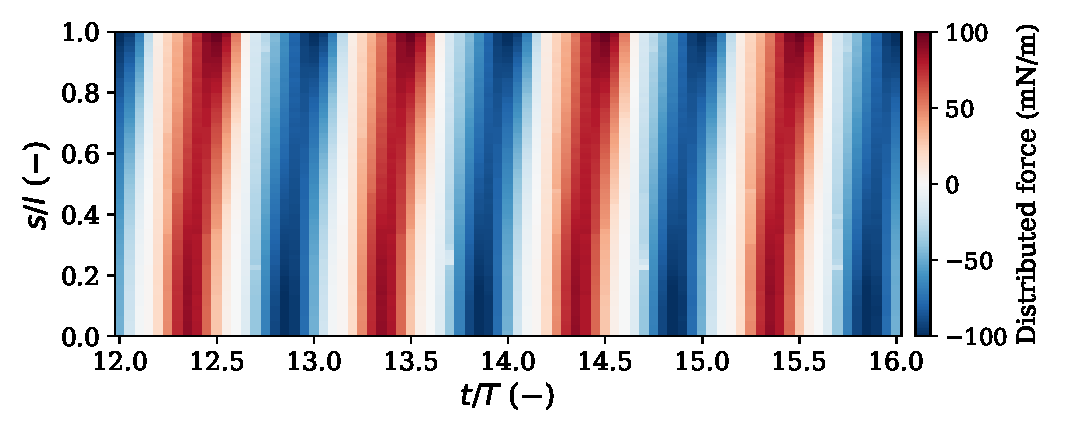
\includegraphics[width=\linewidth]{mimic3_force_heatmap_cd4.pdf}
  \caption{}
\end{subfigure}\hfill
\begin{subfigure}[b]{0.49\textwidth}
  \centering
  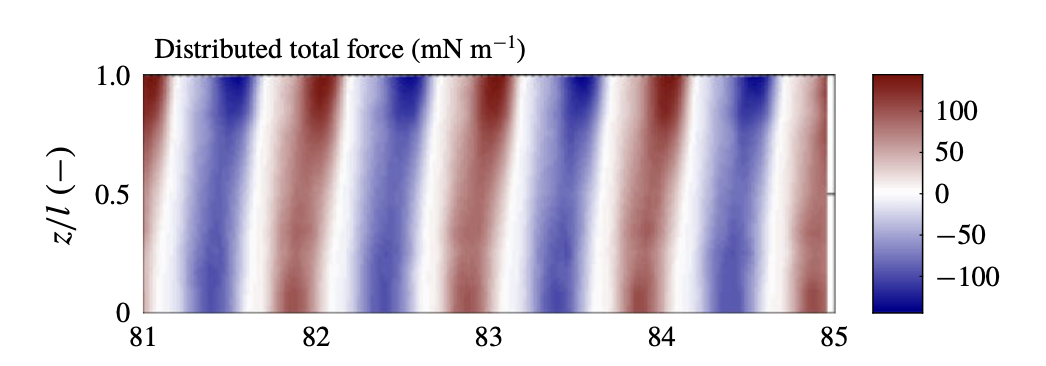
\includegraphics[width=\linewidth]{jacobsen_fig14a.png}
  \caption{}
\end{subfigure}\\[0.4em]
\begin{subfigure}[b]{0.49\textwidth}
  \centering
  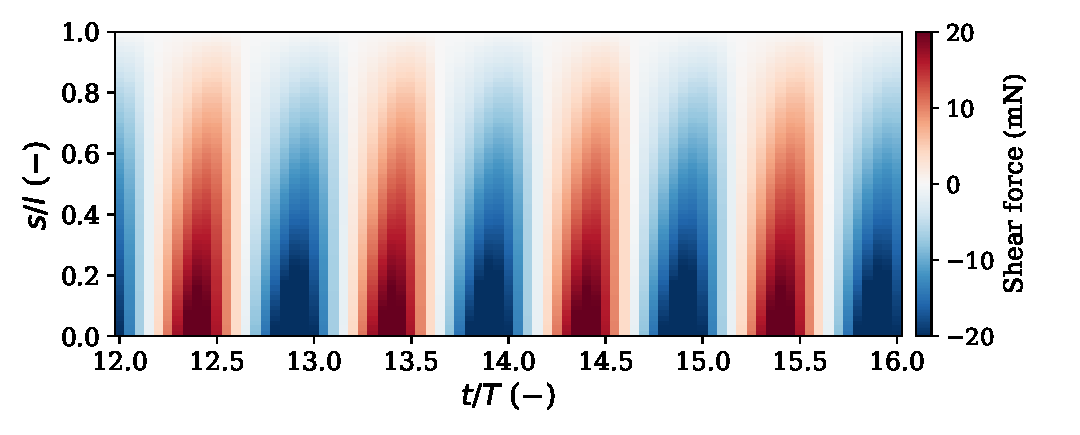
\includegraphics[width=\linewidth]{mimic3_shear_heatmap_cd4.pdf}
  \caption{}
\end{subfigure}\hfill
\begin{subfigure}[b]{0.49\textwidth}
  \centering
  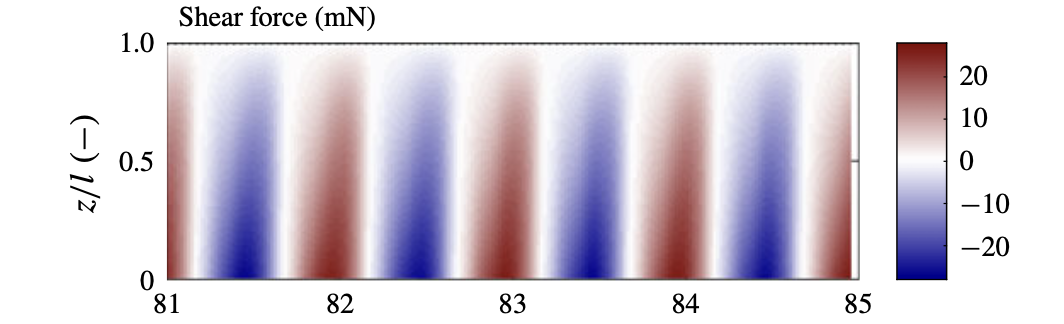
\includegraphics[width=\linewidth]{jacobsen_fig14c.png}
  \caption{}
\end{subfigure}
\caption{Space--time structure of the hydrodynamic loading over four developed wave periods. (a) Actuator-line force per unit length on the stem in the $C_{dn} = 4.0$ simulation. (b) The corresponding experimental reconstruction, reproduced from Figure~14(a) of \citet{jacobsen_waveinduced_2019}. (c) Simulated internal shear-force estimate $V_x(s,t) = \int_s^l f_x\,\mathrm{d}s$. (d) The measured shear, reproduced from their Figure~14(c). Colour scales are common within each pair, at $\pm100~\mathrm{mN\,m^{-1}}$ for the force and $\pm20~\mathrm{mN}$ for the shear. The experimental clock starts at $t/T = 81$ and the simulation at $t/T = 12$.}
\label{fig:flexveg_heatmaps}
\end{figure}

\noindent
The simulated distributed force reproduces the structure of the experimental reconstruction. The loading is in phase along the entire stem, seen as vertical bands characteristic of the quasi-static regime, and it is largest near the free tip and near the root with the minimum at mid-length, which reflects the competition between the orbital-velocity profile, largest near the tip, and the relative-velocity reduction where the stem itself moves fastest. The simulated extrema of $\pm100~\mathrm{mN\,m^{-1}}$ coincide with the limits of the experimental colour scale, and the shear map inherits the same phase structure with its magnitude growing monotonically from tip to root.

\noindent
The base force, which is the row $s/l = 0$ of the shear map and physically the quantity measured by the transducer, is shown in Figure~\ref{fig:flexveg_baseforce} for all three coefficients over the final three periods. The experimental reference is the $\pm20~\mathrm{mN}$ extremum of the reconstructed base shear, at which the colour scale of the reference figure saturates, so the measured extremes are bounded below rather than known exactly. The simulated base force oscillates between $+21$ and $-18~\mathrm{mN}$ at $C_{dn} = 3.0$ and between $+24$ and $-26~\mathrm{mN}$ at $4.0$, reaching and modestly exceeding the saturated scale in the same way the reference's own Morison fit does. This force-level agreement contrasts with the displacement comparison, where the range is $15$ to $20\%$ short at the coefficient the experiment best supports, the two differing because force and displacement are related through the full nonlinear balance rather than proportionally.

\begin{figure}[!htb]
\centering
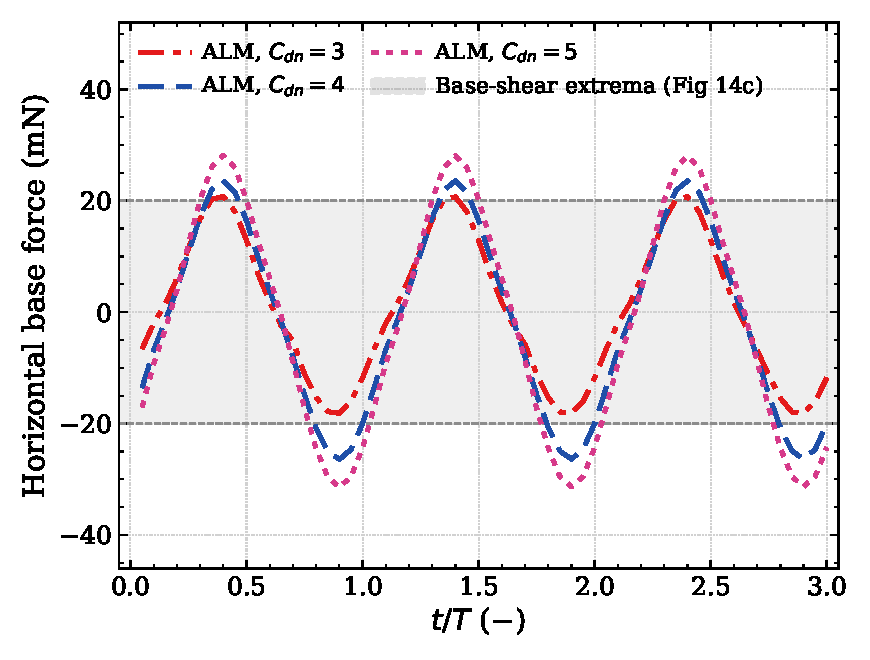
\includegraphics[width=0.66\textwidth]{mimic3_base_force.pdf}
\caption{Horizontal base force over the final three wave periods for the three coefficients, computed as the integral of the distributed actuator-line force along the stem. The shaded band marks $\pm20~\mathrm{mN}$, the extrema of the base-shear reconstruction of \citet[Figure~14c]{jacobsen_waveinduced_2019}, at which their colour scale saturates, so the band is a lower bound on the measured extremes.}
\label{fig:flexveg_baseforce}
\end{figure}

\subsection{Response across the experimental wave conditions}
\label{sec:flexveg_conditions}
The three additional conditions extend the comparison from one point of the experimental parameter space to four, spanning a factor of three in Keulegan--Carpenter number and nearly an order of magnitude in Cauchy number, with the coefficient fixed a priori at each condition. Figure~\ref{fig:flexveg_cond_envelopes} shows the simulated envelopes, and Figure~\ref{fig:flexveg_snapshots} the coupled solution at six phases of a developed wave period for the largest-deflection condition. The tip range grows from $0.096\,l$ for the primary case through $0.18\,l$ and $0.22\,l$ to $0.32\,l$ for the largest wave, at which the stem sweeps through a visibly curved, large-deflection cycle. The geometrically exact formulation and the partitioned coupling handle this progression without adjustment, converging with the same robustness at $0.32\,l$ tip excursion as at $0.096\,l$. In that phase sequence the stem is strongly bent under and just after the crest and relaxes back through the trough phases toward the backward extreme, and the pale streak around and downstream of the stem is the local velocity deficit created by the momentum sink, the footprint of the two-way coupling on the flow. That deficit stays confined to the immediate neighbourhood of the stem and does not disturb the incident wave, consistent with the wave-field verification above.

\begin{figure}[!htb]
\centering
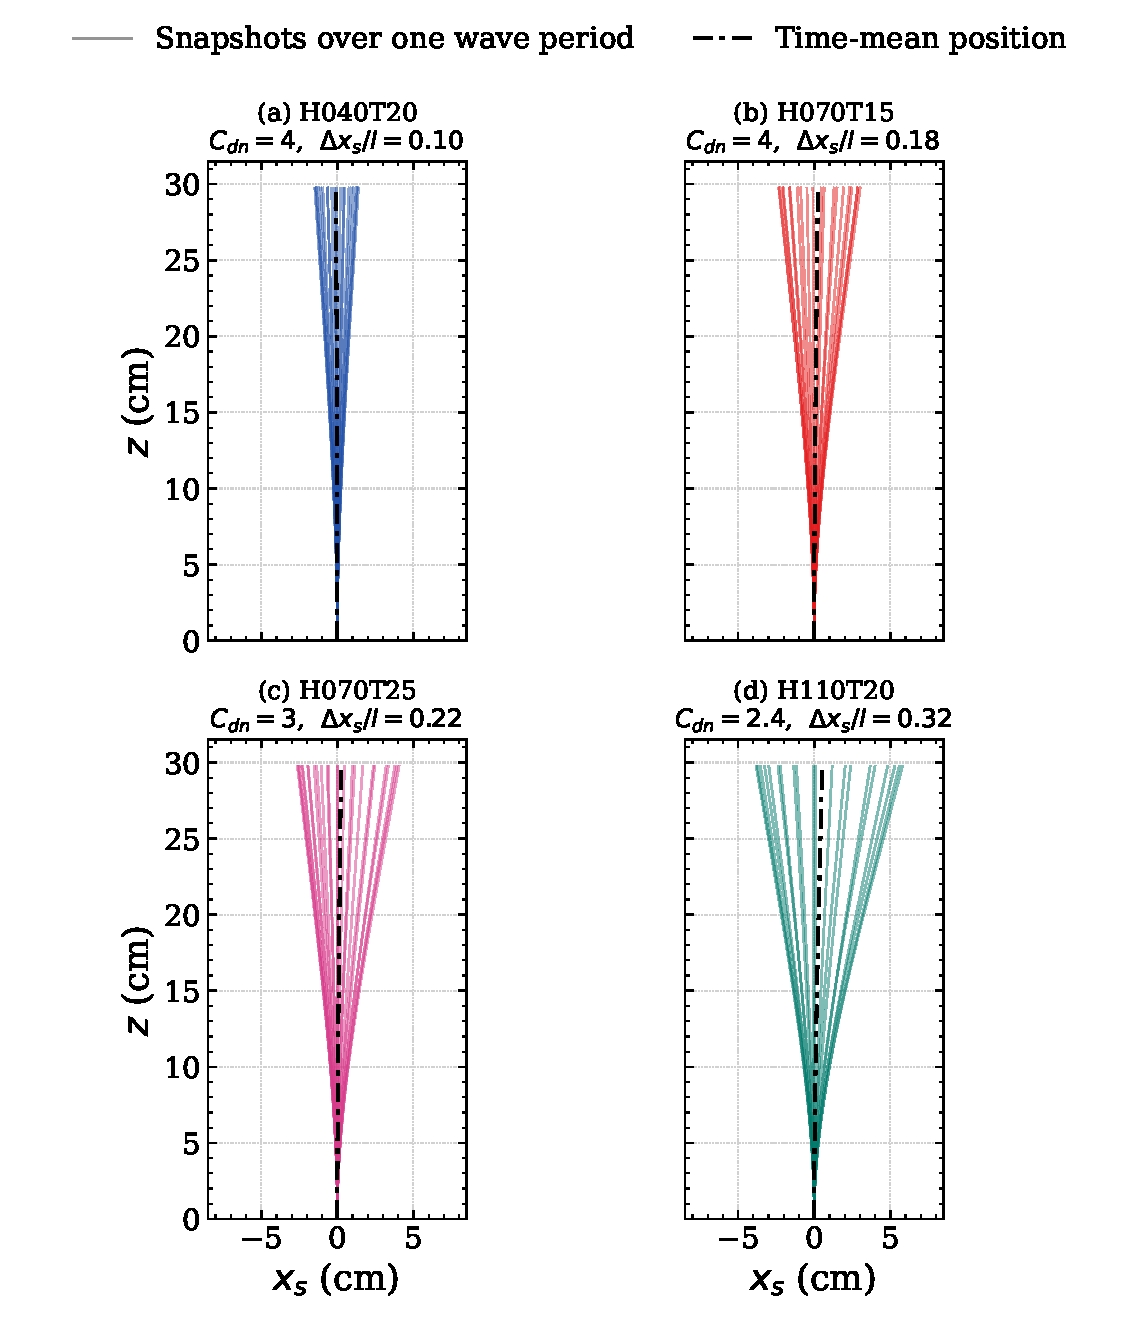
\includegraphics[width=0.68\textwidth]{mimic3_condition_envelopes.pdf}
\caption{Simulated swaying envelopes at the four wave conditions, at the production coefficient of Table~\ref{tab:flexveg_conditions} and with axes true to scale, showing stem centrelines at twenty equispaced instants of one wave period and the time-mean position. The tip oscillation range grows from $0.096\,l$ to $0.32\,l$. No experimental envelope data exist for the three additional conditions.}
\label{fig:flexveg_cond_envelopes}
\end{figure}

\begin{figure}[!htb]
\centering
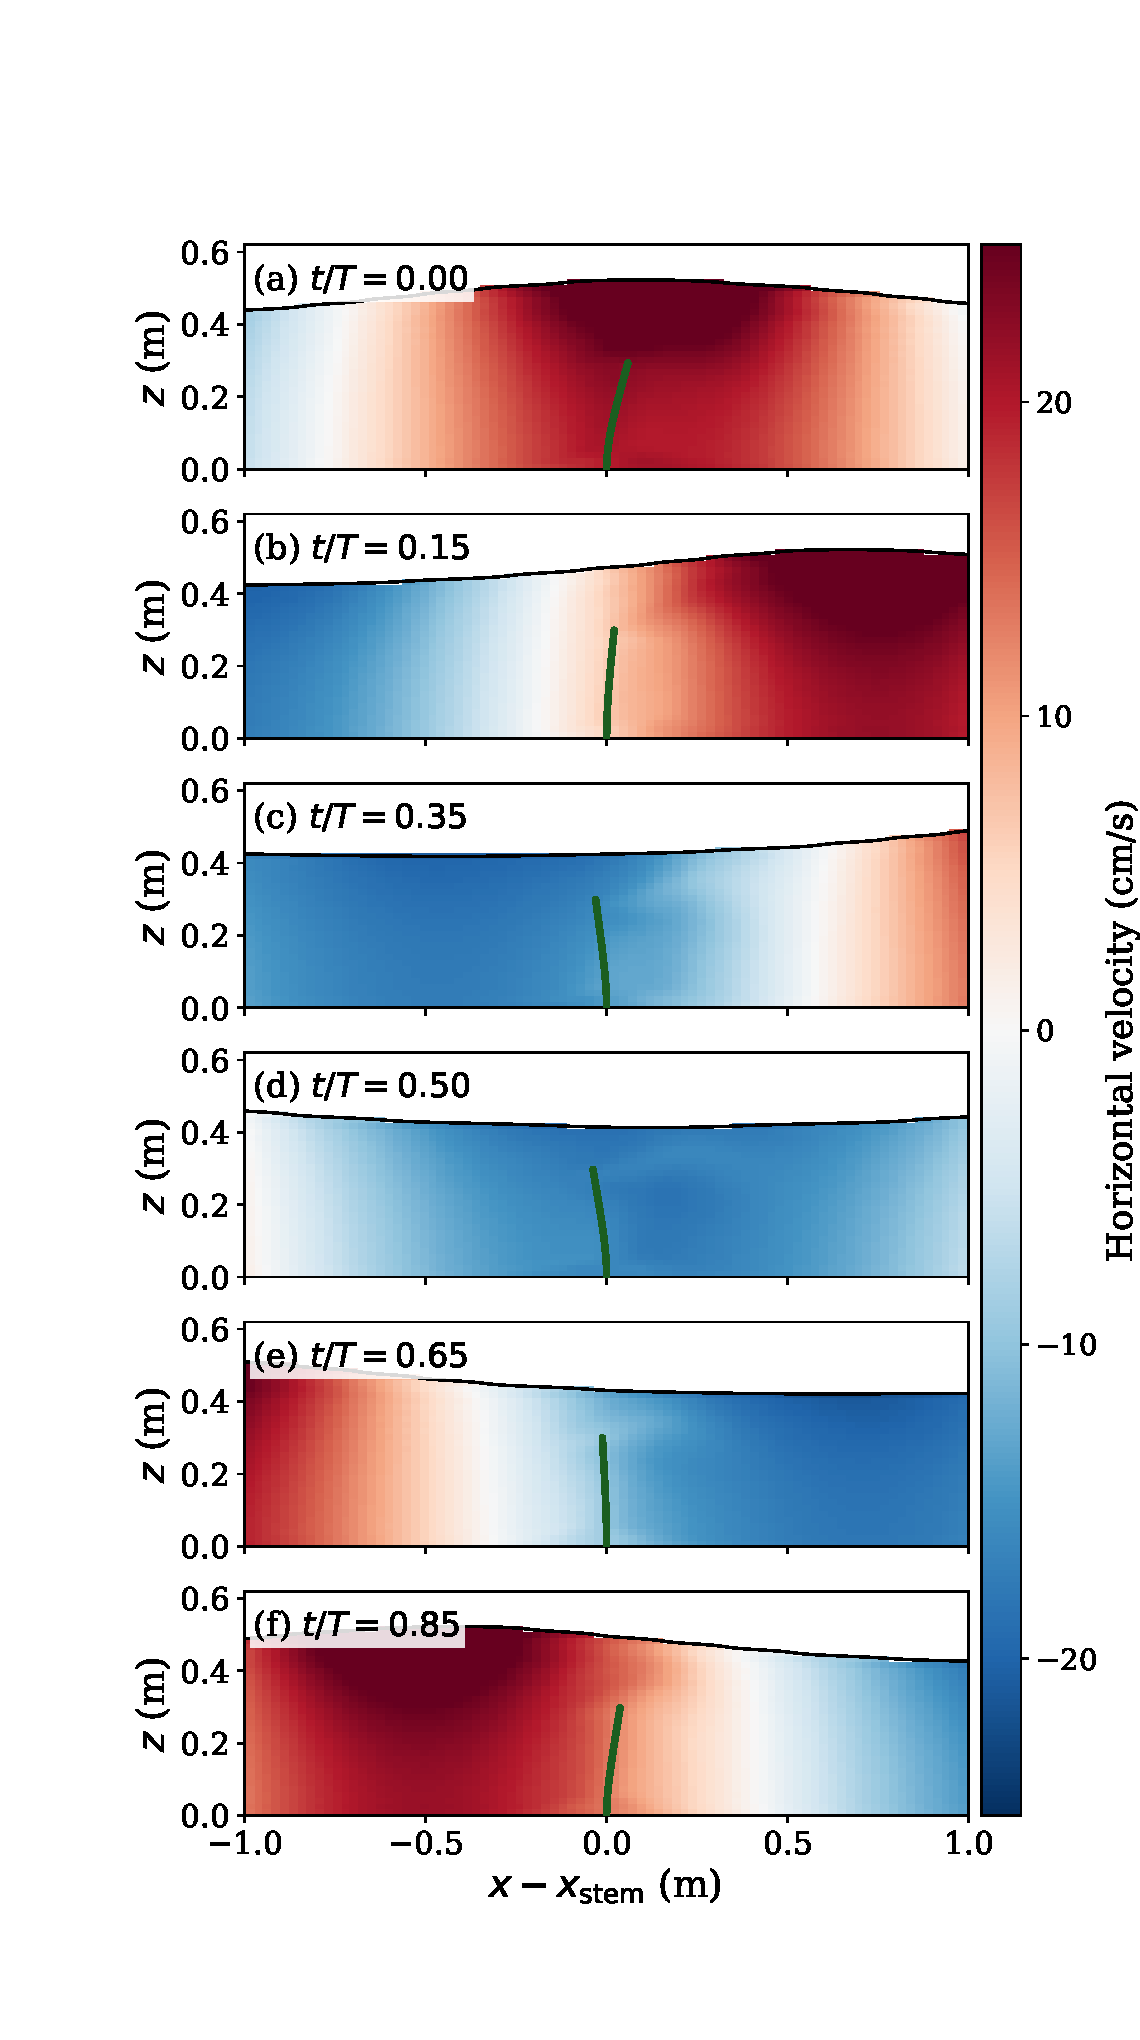
\includegraphics[width=0.50\textwidth]{mimic3_snapshots.pdf}
\caption{Coupled solution at six phases of one developed wave period for the largest-deflection condition H110T20, on the vertical centre plane, showing the horizontal orbital velocity in the water (colour), the free surface (black), and the stem centreline taken from the solver beam-point positions (green). The sequence is anchored at the maximum forward tip deflection and the plotted window covers $\pm1.0~\mathrm{m}$ of the domain around the stem. Every field shown is a solver prediction.}
\label{fig:flexveg_snapshots}
\end{figure}

\noindent
Table~\ref{tab:flexveg_cond_metrics} summarises the scalar outcome against the tip oscillation range normalised by the wave excursion, read for each condition from the tip-motion compilation of the reference. Two captured fractions are quoted. The \emph{raw} fraction compares the simulation directly with the measurement and therefore mixes model error with the input mismatch documented above. The \emph{forcing-corrected} fraction removes that mismatch by normalising the simulated range with the excursion of the wave the simulation actually delivered at the stem, $a_{w}^{\mathrm{sim}} = u_w^{\mathrm{sim}}T/2\pi$, and is the fairer measure of the closure itself. On that measure the three conditions simulated at a coefficient matching its fitted cluster capture $71$ to $83\%$ of the measured response, a consistent level across the full $KC$ range, with no additional degradation appearing at large deflection.

\begin{table}[!ht]
\centering
\small
\caption{Tip response across the four wave conditions. The simulated peak-to-trough tip range, normalised by the wave excursion, against the measured value read from Figure~5 of \citet{jacobsen_waveinduced_2019}. The raw captured fraction uses the experimental $a_w$, and the forcing-corrected fraction normalises the simulation by its own achieved wave excursion. The last column is the amplitude ratio of the quasi-static reconstruction test.}
\label{tab:flexveg_cond_metrics}
\setlength{\tabcolsep}{5pt}
\renewcommand{\arraystretch}{1.15}
\begin{tabular}{l c c c c c c c}
\toprule
Condition & $C_{dn}$ & Tip range$/l$ & $\Delta x_s/a_w$ sim & $\Delta x_s/a_w$ meas & raw & corrected & quasi-static \\
\midrule
H040T20 & $4.0$ & $0.096$ & $1.15$ & $1.41$ & $81\%$ & $83\%$ & $0.98$ \\
H070T15 & $4.0$ & $0.18$ & $1.98$ & $2.41$ & $82\%$ & $71\%$ & $0.97$ \\
H070T25 & $3.0$ & $0.22$ & $1.34$ & $1.48$ & $90\%$ & $81\%$ & $0.98$ \\
H110T20 & $2.4$ & $0.32$ & $1.38$ & $2.21$ & $62\%$ & $71\%$ & $0.97$ \\
\bottomrule
\end{tabular}
\end{table}

\noindent
The boundary probe H070T15 stands outside that quantitative set on two independent grounds, its coefficient having been deliberately chosen above its own cluster and its local wave carrying the reflection contamination quantified above, so its fraction is reported for completeness but not counted toward the closure-accuracy claim. At $CaL/KC = 0.241$, just beyond the quasi-static limit, the experiment shows the largest normalised response of the four conditions, which is the onset of the dynamic amplification that the added-mass inertia provides and that the drag-only closure cannot reproduce. The simulation captures $71\%$ of it on the corrected measure, and even that required a coefficient at the upper edge of the fitted cluster. The shortfall is the expected signature of the closure limitation, in the same direction as the leaflet cases at $\mathrm{St} = 0.5$, but a sharper claim is not possible because the numerical flume is least clean here and the measured deficit mixes the closure limitation with a wave-quality artefact.

\noindent
By itself, an amplitude deficit does not indicate where the model needs improving, since the shortfall could originate anywhere along the chain that produces the response, from the wave generation, through the drag closure and its operators, to the beam solver and its discretisation. The final test isolates the structural end of that chain. For each condition, the tip displacement of the coupled solution is compared in Figure~\ref{fig:flexveg_quasistatic} with a quasi-static reconstruction, in which the instantaneous actuator-line load is applied segment by segment as static point loads on an analytic linear Euler--Bernoulli cantilever of the same $EI$, with no dynamics at all and no time shift. The reconstruction takes the simulated \emph{load} as given and asks whether the simulated \emph{response} is simply the static deflection under that load, so if the coupled solution carried structural dynamics, resonant amplification, a phase lag behind the load, or artefacts of the beam discretisation and the partitioned coupling, the two curves would separate in amplitude or in phase.

\begin{figure}[!htb]
\centering
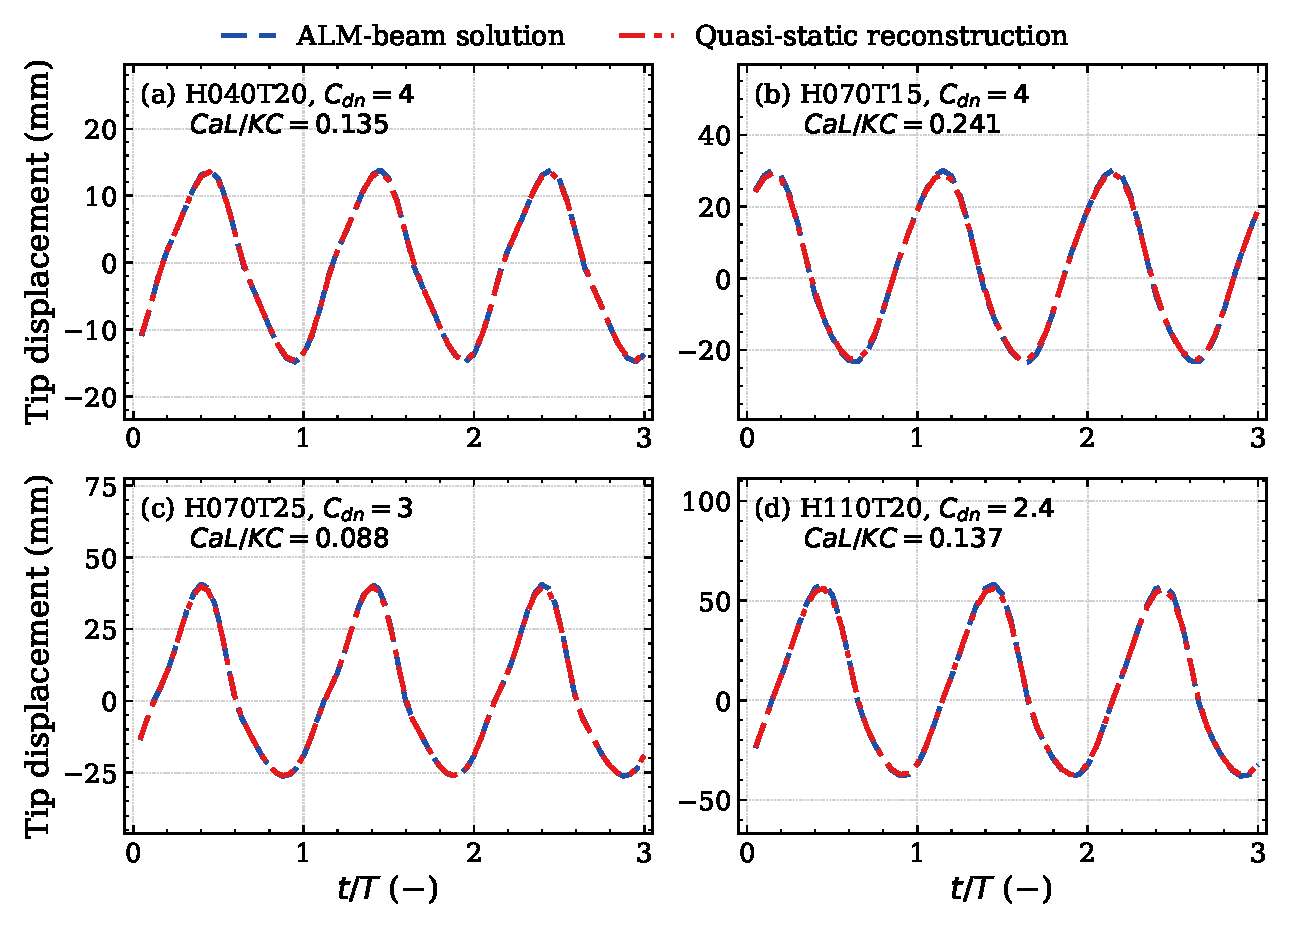
\includegraphics[width=0.92\textwidth]{mimic3_quasistatic.pdf}
\caption{Quasi-static consistency test at the four wave conditions. Tip displacement of the coupled solution against the response of an analytic linear cantilever loaded statically with the instantaneous actuator-line force distribution, with no time shift applied. The reconstruction is in phase and captures $97$ to $98\%$ of the amplitude in every case.}
\label{fig:flexveg_quasistatic}
\end{figure}

\noindent
In all four panels the reconstruction lands on the coupled solution in phase and captures $97$ to $98\%$ of its amplitude, at the largest wave and at the boundary-probe condition alike. The response is therefore quasi-static at all four conditions, exactly as the a priori criterion of Section~\ref{sec:flexveg_case_selection} predicts, so that classification is confirmed numerically rather than only assumed. The $60$-segment beam, the geometrically exact formulation, and the load transmission of the partitioned coupling add no dynamics and no lag of their own and reproduce the amplitude to within $2$ to $3\%$ even at large deflection. The residual deficits therefore sit on the load side of the chain, which covers the quasi-steady closure, the operators that feed and apply it, and the accuracy with which the local wave is reproduced. The test takes the simulated load as given, so it cannot certify that this load is correct, but the wave verification of Section~\ref{sec:flexveg_results_wave} bounds the wave contribution separately, which leaves the closure as the leading candidate for the remainder.

\subsection{Discussion}
\label{sec:flexveg_discussion}
The framework reproduces the shape and the timing of the motion accurately at all four wave conditions. The simulated motion consists of a single spatial mode, in agreement with the decomposition of the measured motion, it is in phase along the whole length of the blade, it shows the correct asymmetry within each wave period, and its mode shape matches the measurement at every drag coefficient tested. The time-mean position is almost exactly vertical, the expected response of a slender blade to symmetric oscillatory forcing when its motion is quasi-static. The distributed force agrees with the experimental reconstruction along the stem and over the wave period and in magnitude, the total force at the base matches the value inferred from the transducer, and at the upper end of the measured coefficient range the positive tip excursion of the primary case is reproduced to within $1\%$.

\noindent
The single feature that the framework does not reproduce accurately is the amplitude of the oscillation, recovering $65$ to $89\%$ of the measured amplitude at the primary condition across the two coefficients, four stations, and two experimental datasets, and $71$ to $83\%$ of the measured tip response across the three quasi-static conditions once the target-versus-achieved wave difference is removed. Increasing the drag coefficient does not remove the shortfall. Raising $C_{dn}$ from $3.0$ to $4.0$ moves across the whole range the experiment fitted to its own measured force, and even that raises the reproduced amplitude only from $65\%$ to $81\%$, while recovering the full measured amplitude would require $5.0$, about $25\%$ larger than the highest value the experiment reports. The response grows more slowly than the coefficient because two effects oppose it, the stem following the surrounding water more closely as the drag becomes stronger, which reduces the relative velocity that generates the drag, and the force applied back to the fluid removing momentum from the local flow, the wave-crest velocity at the stem being lower at $C_{dn} = 4.0$ than at $3.0$. The missing $15$ to $20\%$ is therefore due to physics that the closure does not represent rather than to an incorrect coefficient, and the most likely source is the fluid-inertia force, which the reference's own force decomposition places below $10\%$ of the maximum force for this stem. The same limitation was identified in the leaflet benchmark at a Strouhal number of $0.5$, and it is now confirmed against a physical experiment rather than a reference simulation. The quasi-static reconstruction locates it, since the structural side reproduces the coupled response to within $2$ to $3\%$ in amplitude and exactly in phase at all four conditions.

\noindent
Two features of the experiment limit the precision of the comparison across conditions. The published wave kinematics describe the waves the flume actually generated, which exceed their nominal targets by as much as $17\%$, whereas the simulations are driven by the target waves, and the forcing-corrected column accounts for this only to first order because the correction is based on the wave kinematics alone. At H070T15 the outlet absorption also operates close to the limit of its shallow-water validity and admits a weak reflected wave, so the comparison there is qualitative, the shortfall having the expected sign and magnitude but not separating cleanly into the part caused by the closure and the part caused by the imperfect wave.

\noindent
It is finally useful to place the result beside the most detailed simulation of the same experiment available. \citet{prueter_vegetation_2025} coupled a geometrically exact rod to a fully resolved two-phase flow and simulated the same campaign at the primary wave condition, using the thinner Mimic~2 blade whose response lies in the dynamic regime deliberately excluded here. Their model resolves the added-mass force that the present closure omits and reproduces the tip position of that blade with an average error of about $6$ to $7\%$ of the stem length, but it does not recover the measured mean forward drift or the second mode of the dynamic response. Because the two studies use different blades the comparison is indicative rather than exact, but for the quasi-static conditions considered here a drag-only actuator-line model reaches an accuracy of the same order as a fully resolved method achieves on the more demanding dynamic blade, with an error budget that separates clearly into the coefficient range, the wave quality, and the missing closure physics. A direct comparison of computational cost would require both studies to be run with the same hardware, tolerances, durations, and accuracy targets, none of which the published work reports. What can be reported is the cost of the present simulations, approximately six days of wall-clock time on $256$ cores for each wave condition, using about $1.35\times10^{7}$ fluid cells and $6.4\times10^{5}$ time steps, with the small step set by the beam solver rather than by the fluid. The actuator-line representation requires neither a body-conforming mesh around the millimetre-scale cross-section nor any mesh motion, so its cost is expected to grow far more slowly than that of a fully resolved method as the number of stems increases, which is the setting the framework is intended for, accepting a known amplitude error of $15$ to $20\%$ per stem in exchange.

